\documentclass[letter,10pt,twoside]{article}

\usepackage[spanish,es-nodecimaldot]{babel}
\usepackage[utf8]{inputenc}

\renewcommand{\familydefault}{\sfdefault}
\usepackage[T1]{fontenc}
\usepackage{textcomp}

\usepackage{framed}
\usepackage[svgnames]{xcolor}
\colorlet{shadecolor}{Gainsboro!50}

\usepackage{enumitem}
\usepackage{graphicx}
\usepackage{pstricks}

\usepackage{anysize}
\marginsize{3cm}{2cm}{2cm}{3cm}

\usepackage{float}
\usepackage{siunitx}
\usepackage{amsmath}
\usepackage{array}

\usepackage{multicol}
\usepackage{pifont}

\usepackage{fancyhdr}
\usepackage{lastpage}
\pagestyle{fancy}
\fancyhf{}
\fancyhead[LE,RO]{Resistencia de los Materiales}
\fancyfoot[CO,CE]{\thepage\ de \pageref{LastPage}}

\special{papersize=215.9mm,279.4mm}

\usepackage[
    pdfauthor={Carlos Eduardo Caballero Burgoa},%
    pdftitle={Resistencia de los Materiales},%
    pdfsubject={Practica 01},%
    colorlinks,%
    citecolor=black,%
    filecolor=black,%
    linkcolor=black,%
    urlcolor=black,
    breaklinks]{hyperref}
\usepackage{breakurl}

\newcommand{\blankpage}{
\newpage
\thispagestyle{empty}
\mbox{}
\newpage
}

\renewcommand{\arraystretch}{1.2}

\begin{document}

\begin{titlepage}
\begin{center}
{\Large UNIVERSIDAD MAYOR DE SAN SIMÓN}\\
\vspace*{0.15cm}
{\large FACULTAD DE CIENCIAS Y TECNOLOGÍA}\\
\vspace*{9.0cm}
{\Large \textbf{PRACTICA No. 1}}\\
\end{center}

\vspace*{7.4cm}
\leftskip=7.95cm
\noindent
\textbf{Estudiante:}\\
Caballero Burgoa, Carlos Eduardo.\\
\textbf{Carrera:}\\
Ingeniería Electromecánica.\\
\newline
\textbf{Docente:}\\
Ing. Guido Gomez Ugarte.\\
\newline
\textbf{Fecha de entrega:} 20 de Septiembre del 2022.\\

\end{titlepage}

\blankpage

\colorbox{blue!25}{\textbf{PROBLEMA 1:}}

\begin{figure}[H]
\centering
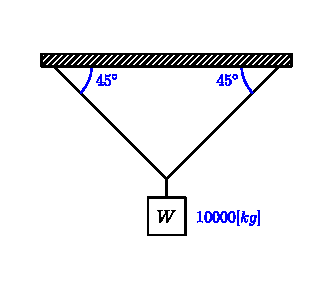
\includegraphics[scale=1.3]{resources/f01.eps}
\end{figure}

\textbf{\underline{Solución}:} \\

\textbf{Sistema concurrente:} \\
Se plantean las ecuaciones de equilibrio:

\begin{equation*}
    \sum{F_x} = 0
\end{equation*}
\begin{equation*}
    \sum{F_y} = 0
\end{equation*}

\begin{figure}[H]
\centering
\includegraphics[scale=1.3]{resources/g01.eps}
\end{figure}

\textbf{Variables:} $T_1$, $T_2$.
\\

$\sum{F_x} = 0$:
\begin{equation*}
    T_{1x} - T_{2x} = 0
\end{equation*}
\begin{equation*}
    T_1\,cos(45^\circ) - T_2\,cos(45^\circ) = 0
\end{equation*}

$\sum{F_y} = 0$:
\begin{equation*}
    T_{1y} + T_{2y} - W = 0
\end{equation*}
\begin{equation*}
    T_1\,sen(45^\circ) + T_2\,sen(45^\circ) = 10000
\end{equation*}

Resolviendo el sistema de ecuaciones lineales 2x2:

\begin{equation*}
\boxed{
    \begin{array}{l}
        T_1 = 707.11[\text{kg}] \\
        T_2 = 707.11[\text{kg}]
    \end{array}
}
\end{equation*}

Por tanto:

\begin{equation*}
\boxed{
    \begin{array}{l}
        \text{Sistema isoestático}
    \end{array}
}
\end{equation*}

\vspace{1.0cm}

\colorbox{blue!25}{\textbf{PROBLEMA 2:}}

\begin{figure}[H]
\centering
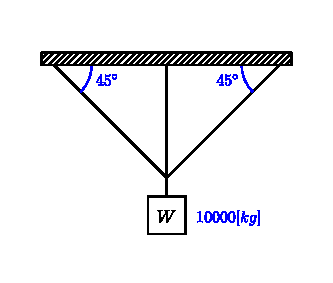
\includegraphics[scale=1.3]{resources/f02.eps}
\end{figure}

\textbf{\underline{Solución}:} \\

\textbf{Sistema concurrente:} \\
Se plantean las ecuaciones de equilibrio:

\begin{equation*}
    \sum{F_x} = 0
\end{equation*}
\begin{equation*}
    \sum{F_y} = 0
\end{equation*}

\begin{figure}[H]
\centering
\includegraphics[scale=1.3]{resources/g02.eps}
\end{figure}

\textbf{Variables:} $T_1$, $T_2$, $T_3$.
\\

$\sum{F_x} = 0$:
\begin{equation*}
    T_{1x} - T_{3x} = 0
\end{equation*}
\begin{equation*}
    T_1\,cos(45^\circ) - T_3\,cos(45^\circ) = 0
\end{equation*}

$\sum{F_y} = 0$:
\begin{equation*}
    T_{1y} + T_2 + T_{3y} - W = 0
\end{equation*}
\begin{equation*}
    T_1\,sen(45^\circ) + T_2 + T_3\,sen(45^\circ) = 10000
\end{equation*}

Se tienen 2 ecuaciones para 3 incógnitas.

Por tanto:

\begin{equation*}
\boxed{
    \begin{array}{l}
        \text{Sistema hiperestático}
    \end{array}
}
\end{equation*}

\vspace{1.0cm}

\colorbox{blue!25}{\textbf{PROBLEMA 3:}}

\begin{figure}[H]
\centering
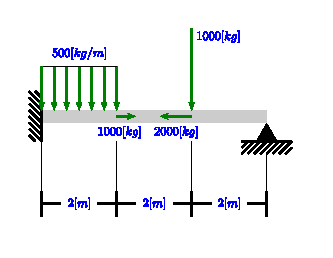
\includegraphics[scale=1.8]{resources/f03.eps}
\end{figure}

\textbf{\underline{Solución}:} \\

\textbf{Sistema no concurrente:} \\
Se plantean las ecuaciones de equilibrio:

\begin{equation*}
    \sum{F_x} = 0
\end{equation*}
\begin{equation*}
    \sum{F_y} = 0
\end{equation*}

Se consideran los siguientes puntos para el calculo de momentos:

\begin{figure}[H]
\centering
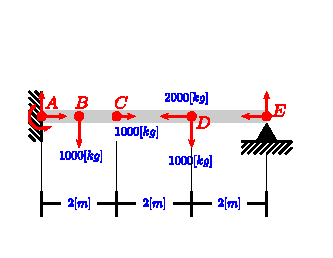
\includegraphics[scale=1.8]{resources/g03.eps}
\end{figure}

\begin{equation*}
    \sum{M_A} = 0
\end{equation*}
\begin{equation*}
    \sum{M_B} = 0
\end{equation*}
\begin{equation*}
    \sum{M_C} = 0
\end{equation*}
\begin{equation*}
    \sum{M_D} = 0
\end{equation*}
\begin{equation*}
    \sum{M_E} = 0
\end{equation*}

\textbf{Variables:} $A_x$, $A_y$, $M_A$, $E_x$, $E_y$.
\\

\begin{figure}[H]
\centering
\includegraphics[scale=1.8]{resources/h03.eps}
\end{figure}

$\sum{F_x} = 0$:
\begin{equation*}
    A_x + 1000 - E_x - 2000 = 0
\end{equation*}
\begin{equation*}
    A_x - E_x = 1000
\end{equation*}

$\sum{F_y} = 0$:
\begin{equation*}
    A_y - 1000 - 1000 + E_y = 0
\end{equation*}
\begin{equation*}
    A_y + E_y = 2000
\end{equation*}

$\sum{M_A} = 0$:
\begin{equation*}
    - M_A + 1000(1) + 1000(4) - E_y(6) = 0
\end{equation*}
\begin{equation*}
    M_A + 6E_y = 5000
\end{equation*}

$\sum{M_B} = 0$:
\begin{equation*}
    - M_A + A_y(1) + 1000(3) - E_y(5) = 0
\end{equation*}
\begin{equation*}
    - M_A + A_y - 5 E_y = -3000
\end{equation*}

$\sum{M_C} = 0$:
\begin{equation*}
    - M_A + A_y(2) - 1000(1) + 1000(2) - E_y(4) = 0
\end{equation*}
\begin{equation*}
    - M_A + 2 A_y - 4 E_y = -1000
\end{equation*}

$\sum{M_D} = 0$:
\begin{equation*}
    - M_A + A_y(4) - 1000(3) - E_y(2) = 0
\end{equation*}
\begin{equation*}
    - M_A + 4 A_y - 2 E_y = 3000
\end{equation*}

$\sum{M_E} = 0$:
\begin{equation*}
    - M_A + A_y (6) - 1000(5) - 1000(2) = 0
\end{equation*}
\begin{equation*}
    - M_A + 6 A_y = 7000
\end{equation*}

Resolviendo las ecuaciones, se obtienen infinitas soluciones.

Por tanto:

\begin{equation*}
\boxed{
    \begin{array}{l}
        \text{Sistema hiperestático}
    \end{array}
}
\end{equation*}

\vspace{1.0cm}

\colorbox{blue!25}{\textbf{PROBLEMA 4:}}

\begin{figure}[H]
\centering
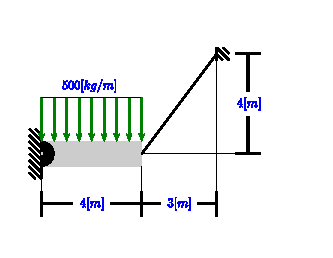
\includegraphics[scale=1.8]{resources/f04.eps}
\end{figure}

\textbf{\underline{Solución}:} \\

\textbf{Sistema no concurrente:} \\
Se plantean las ecuaciones de equilibrio:

\begin{equation*}
    \sum{F_x} = 0
\end{equation*}
\begin{equation*}
    \sum{F_y} = 0
\end{equation*}

Se consideran los siguientes puntos para el calculo de momentos:

\begin{figure}[H]
\centering
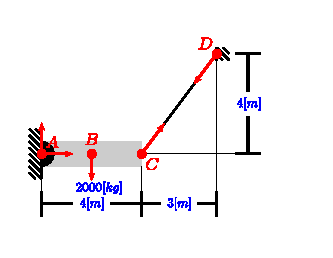
\includegraphics[scale=1.8]{resources/g04.eps}
\end{figure}

\begin{equation*}
    \sum{M_A} = 0
\end{equation*}
\begin{equation*}
    \sum{M_B} = 0
\end{equation*}
\begin{equation*}
    \sum{M_C} = 0
\end{equation*}

\textbf{Variables:} $A_x$, $A_y$, $T$.
\\

\begin{figure}[H]
\centering
\includegraphics[scale=1.8]{resources/h04.eps}
\end{figure}

$\sum{F_x} = 0$:
\begin{equation*}
    A_x + T_x = 0
\end{equation*}
\begin{equation*}
    A_x + \frac{3}{5} T = 0
\end{equation*}

$\sum{F_y} = 0$:
\begin{equation*}
    A_y - 2000 + T_y = 0
\end{equation*}
\begin{equation*}
    A_y + \frac{4}{5} T = 2000
\end{equation*}

$\sum{M_A} = 0$:
\begin{equation*}
    2000(2) - T_y(4) = 0
\end{equation*}
\begin{equation*}
    \frac{16}{5} T = 4000
\end{equation*}

$\sum{M_B} = 0$:
\begin{equation*}
    A_y(2) - T_y(2) = 0
\end{equation*}
\begin{equation*}
    2 A_y - \frac{8}{5} T = 0
\end{equation*}

$\sum{M_C} = 0$:
\begin{equation*}
    A_y(4) - 2000(2) = 0
\end{equation*}
\begin{equation*}
    4 A_y = 4000
\end{equation*}

Resolviendo el sistema de ecuaciones lineales 3x3:

\begin{equation*}
\boxed{
    \begin{array}{l}
        T = 1250[\text{kg}] \\
        A_x = 750[\text{kg}] \\
        A_y = 1000[\text{kg}]
    \end{array}
}
\end{equation*}

Por tanto:

\begin{equation*}
\boxed{
    \begin{array}{l}
        \text{Sistema isoestático}
    \end{array}
}
\end{equation*}

\vspace{1.0cm}

\colorbox{blue!25}{\textbf{PROBLEMA 5:}}

\begin{figure}[H]
\centering
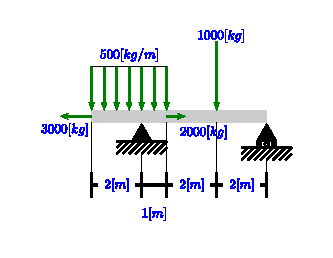
\includegraphics[scale=1.8]{resources/f05.eps}
\end{figure}

\textbf{\underline{Solución}:} \\

\textbf{Sistema no concurrente:} \\
Se plantean las ecuaciones de equilibrio:

\begin{equation*}
    \sum{F_x} = 0
\end{equation*}
\begin{equation*}
    \sum{F_y} = 0
\end{equation*}

Se consideran los siguientes puntos para el calculo de momentos:

\begin{figure}[H]
\centering
\includegraphics[scale=1.8]{resources/g05.eps}
\end{figure}

\begin{equation*}
    \sum{M_A} = 0
\end{equation*}
\begin{equation*}
    \sum{M_B} = 0
\end{equation*}
\begin{equation*}
    \sum{M_C} = 0
\end{equation*}
\begin{equation*}
    \sum{M_D} = 0
\end{equation*}
\begin{equation*}
    \sum{M_E} = 0
\end{equation*}
\begin{equation*}
    \sum{M_F} = 0
\end{equation*}

\textbf{Variables:} $C_x$, $C_y$, $F_y$.
\\

\begin{figure}[H]
\centering
\includegraphics[scale=1.8]{resources/h05.eps}
\end{figure}

$\sum{F_x} = 0$:
\begin{equation*}
    -3000 - C_x + 2000 = 0
\end{equation*}
\begin{equation*}
    C_x = -1000
\end{equation*}

$\sum{F_y} = 0$:
\begin{equation*}
    -1500 + C_y - 1000 + F_y = 0
\end{equation*}
\begin{equation*}
    C_y + F_y = 2500
\end{equation*}

$\sum{M_A} = 0$:
\begin{equation*}
    1500(1.5) - C_y(2) + 1000(5) - F_y(7) = 0
\end{equation*}
\begin{equation*}
    2 C_y + 7 F_y = 7250
\end{equation*}

$\sum{M_B} = 0$:
\begin{equation*}
    C_y(0.5) - 1000(3.5) + F_y(5.5) = 0
\end{equation*}
\begin{equation*}
    0.5 C_y + 5.5 F_y = 3500
\end{equation*}

$\sum{M_C} = 0$:
\begin{equation*}
    -1500(0.5) + 1000(3) - F_y(5) = 0
\end{equation*}
\begin{equation*}
    5 F_y = 2250
\end{equation*}

$\sum{M_D} = 0$:
\begin{equation*}
    -1500(1.5) + C_y(1) + 1000(2) - F_y(4) = 0
\end{equation*}
\begin{equation*}
    C_y - 4 F_y = 250
\end{equation*}

$\sum{M_E} = 0$:
\begin{equation*}
    -1500(3.5) + C_y(3) - F_y(2) = 0
\end{equation*}
\begin{equation*}
    3 C_y - 2 F_y = 5250
\end{equation*}

$\sum{M_F} = 0$:
\begin{equation*}
    -1500(5.5) + C_y(5) - 1000(2) = 0
\end{equation*}
\begin{equation*}
    5 C_y = 10250
\end{equation*}

Resolviendo las ecuaciones, se obtiene:

\begin{equation*}
\boxed{
    \begin{array}{l}
        C_x = -1000[\text{kg}] \\
        C_y = 2050[\text{kg}] \\
        F_y = 450[\text{kg}]
    \end{array}
}
\end{equation*}

Por tanto:

\begin{equation*}
\boxed{
    \begin{array}{l}
        \text{Sistema isoestático}
    \end{array}
}
\end{equation*}

\vspace{1.0cm}

\colorbox{blue!25}{\textbf{PROBLEMA 6:}}

\begin{figure}[H]
\centering
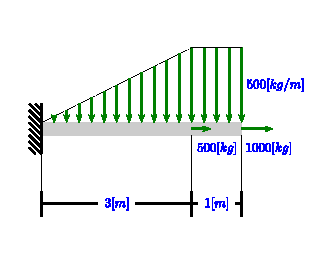
\includegraphics[scale=1.8]{resources/f06.eps}
\end{figure}

\textbf{\underline{Solución}:} \\

\textbf{Sistema no concurrente:} \\
Se plantean las ecuaciones de equilibrio:

\begin{equation*}
    \sum{F_x} = 0
\end{equation*}
\begin{equation*}
    \sum{F_y} = 0
\end{equation*}

Se consideran los siguientes puntos para el calculo de momentos:

\begin{figure}[H]
\centering
\includegraphics[scale=1.8]{resources/g06.eps}
\end{figure}

\begin{equation*}
    \sum{M_A} = 0
\end{equation*}
\begin{equation*}
    \sum{M_B} = 0
\end{equation*}
\begin{equation*}
    \sum{M_C} = 0
\end{equation*}
\begin{equation*}
    \sum{M_D} = 0
\end{equation*}
\begin{equation*}
    \sum{M_E} = 0
\end{equation*}

\textbf{Variables:} $A_x$, $A_y$, $M_A$.
\\

\begin{figure}[H]
\centering
\includegraphics[scale=1.8]{resources/h06.eps}
\end{figure}

$\sum{F_x} = 0$:
\begin{equation*}
    A_x + 500 + 1000 = 0
\end{equation*}
\begin{equation*}
    A_x = -1500
\end{equation*}

$\sum{F_y} = 0$:
\begin{equation*}
    A_y - 750 - 500 = 0
\end{equation*}
\begin{equation*}
    A_y = 1250
\end{equation*}

$\sum{M_A} = 0$:
\begin{equation*}
    - M_A + 750(2) + 500(3.5) = 0
\end{equation*}
\begin{equation*}
    M_A = 3250
\end{equation*}

$\sum{M_B} = 0$:
\begin{equation*}
    - M_A + A_y(2) + 500(1.5) = 0
\end{equation*}
\begin{equation*}
    - M_A + 2 A_y = -750
\end{equation*}

$\sum{M_C} = 0$:
\begin{equation*}
    - M_A + A_y(3) - 750(1) + 500(0.5) = 0
\end{equation*}
\begin{equation*}
    - M_A + 3 A_y = 500
\end{equation*}

$\sum{M_D} = 0$:
\begin{equation*}
    - M_A + A_y(3.5) - 750(1.5) = 0
\end{equation*}
\begin{equation*}
    - M_A + 3.5 A_y = 1125
\end{equation*}

$\sum{M_E} = 0$:
\begin{equation*}
    - M_A + A_y(4) - 750(2) - 500(0.5) = 0
\end{equation*}
\begin{equation*}
    - M_A + 4 A_y = 1750
\end{equation*}

Resolviendo las ecuaciones, se obtiene:

\begin{equation*}
\boxed{
    \begin{array}{l}
        A_x = -1500[\text{kg}] \\
        A_y = 1250[\text{kg}] \\
        M_A = 3250[\text{kg-m}]
    \end{array}
}
\end{equation*}

Por tanto:

\begin{equation*}
\boxed{
    \begin{array}{l}
        \text{Sistema isoestático}
    \end{array}
}
\end{equation*}

\vspace{1.0cm}

\colorbox{blue!25}{\textbf{PROBLEMA 7:}}

\begin{figure}[H]
\centering
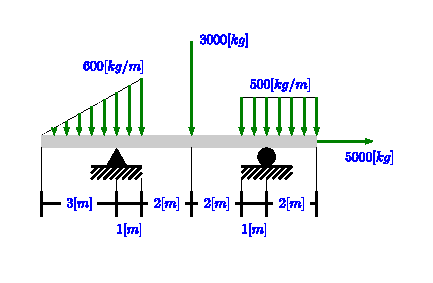
\includegraphics[scale=1.8]{resources/f07.eps}
\end{figure}

\textbf{\underline{Solución}:} \\

\textbf{Sistema no concurrente:} \\
Se plantean las ecuaciones de equilibrio:

\begin{equation*}
    \sum{F_x} = 0
\end{equation*}
\begin{equation*}
    \sum{F_y} = 0
\end{equation*}

Se consideran los siguientes puntos para el calculo de momentos:

\begin{figure}[H]
\centering
\includegraphics[scale=1.8]{resources/g07.eps}
\end{figure}

\begin{equation*}
    \sum{M_A} = 0
\end{equation*}
\begin{equation*}
    \sum{M_B} = 0
\end{equation*}
\begin{equation*}
    \sum{M_C} = 0
\end{equation*}
\begin{equation*}
    \sum{M_D} = 0
\end{equation*}
\begin{equation*}
    \sum{M_E} = 0
\end{equation*}
\begin{equation*}
    \sum{M_F} = 0
\end{equation*}
\begin{equation*}
    \sum{M_G} = 0
\end{equation*}

\textbf{Variables:} $C_x$, $C_y$, $E_y$.
\\

\begin{figure}[H]
\centering
\includegraphics[scale=1.8]{resources/h07.eps}
\end{figure}

$\sum{F_x} = 0$:
\begin{equation*}
    C_x - 5000 = 0
\end{equation*}
\begin{equation*}
    C_x = 5000
\end{equation*}

$\sum{F_y} = 0$:
\begin{equation*}
    -1200 + C_y - 3000 + E_y -1500 = 0
\end{equation*}
\begin{equation*}
    C_y + E_y = 5700
\end{equation*}

$\sum{M_A} = 0$:
\begin{equation*}
    1200(4)(\frac{2}{3}) - C_y(3) + 3000(6) - E_y(9) + 1500(9.5) = 0
\end{equation*}
\begin{equation*}
    3 C_y + 9 E_y = 35450
\end{equation*}

$\sum{M_B} = 0$:
\begin{equation*}
    - C_y(\frac{1}{3}) + 3000(\frac{10}{3}) - E_y(\frac{19}{3}) + 1500(\frac{41}{6}) = 0
\end{equation*}
\begin{equation*}
    \frac{1}{3}C_y + \frac{19}{3} E_y = 20250
\end{equation*}

$\sum{M_C} = 0$:
\begin{equation*}
    -1200(\frac{1}{3}) + 3000(3) - E_y(6) + 1500(6.5) = 0
\end{equation*}
\begin{equation*}
    E_y = 3058.33
\end{equation*}

$\sum{M_D} = 0$:
\begin{equation*}
    -1200(\frac{10}{3}) + C_y(3) - E_y(3) + 1500(3.5) = 0
\end{equation*}
\begin{equation*}
    3 C_y - 3 E_y = -1250
\end{equation*}

$\sum{M_E} = 0$:
\begin{equation*}
    -1200(\frac{19}{3}) + C_y(6) - 3000(3) + 1500(0.5) = 0
\end{equation*}
\begin{equation*}
    C_y = 2641.67
\end{equation*}

$\sum{M_F} = 0$:
\begin{equation*}
    -1200(\frac{41}{6}) + C_y(6.5) - 3000(3.5) + E_y(0.5) = 0
\end{equation*}
\begin{equation*}
    6.5 C_y + 0.5 E_y = 18700
\end{equation*}

$\sum{M_G} = 0$:
\begin{equation*}
    -1200(\frac{25}{3}) + C_y(8) - 3000(5) + E_y(2) -1500(1.5) = 0
\end{equation*}
\begin{equation*}
    8 C_y + 2 E_y = 27250
\end{equation*}

Resolviendo las ecuaciones, se obtiene:

\begin{equation*}
\boxed{
    \begin{array}{l}
        C_x = 5000[\text{kg}] \\
        C_y = 2641.67[\text{kg}] \\
        E_y = 3058.33[\text{kg}]
    \end{array}
}
\end{equation*}

Por tanto:

\begin{equation*}
\boxed{
    \begin{array}{l}
        \text{Sistema isoestático}
    \end{array}
}
\end{equation*}

\vspace{1.0cm}

\colorbox{blue!25}{\textbf{PROBLEMA 8:}}

\begin{figure}[H]
\centering
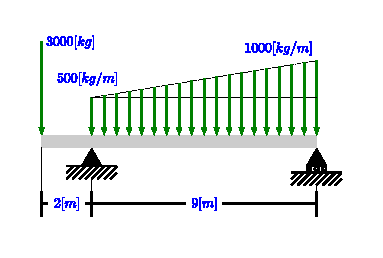
\includegraphics[scale=1.8]{resources/f08.eps}
\end{figure}

\textbf{\underline{Solución}:} \\

\textbf{Sistema no concurrente:} \\
Se plantean las ecuaciones de equilibrio:

\begin{equation*}
    \sum{F_x} = 0
\end{equation*}
\begin{equation*}
    \sum{F_y} = 0
\end{equation*}

Se consideran los siguientes puntos para el calculo de momentos:

\begin{figure}[H]
\centering
\includegraphics[scale=1.8]{resources/g08.eps}
\end{figure}

\begin{equation*}
    \sum{M_A} = 0
\end{equation*}
\begin{equation*}
    \sum{M_B} = 0
\end{equation*}
\begin{equation*}
    \sum{M_C} = 0
\end{equation*}
\begin{equation*}
    \sum{M_D} = 0
\end{equation*}
\begin{equation*}
    \sum{M_E} = 0
\end{equation*}

\textbf{Variables:} $B_x$, $B_y$, $E_y$.
\\

\begin{figure}[H]
\centering
\includegraphics[scale=1.8]{resources/h08.eps}
\end{figure}

$\sum{F_x} = 0$:
\begin{equation*}
    B_x = 0
\end{equation*}

$\sum{F_y} = 0$:
\begin{equation*}
    -3000 + B_y - 4500 - 2250 + E_y = 0
\end{equation*}
\begin{equation*}
    B_y + E_y = 9750
\end{equation*}

$\sum{M_A} = 0$:
\begin{equation*}
    - B_y(2) + 4500(6.5) + 2250(8) - E_y(11) = 0
\end{equation*}
\begin{equation*}
    2 B_y + 11 E_y = 47250
\end{equation*}

$\sum{M_B} = 0$:
\begin{equation*}
    -3000(2) + 4500(4.5) + 2250(6) - E_y(9) = 0
\end{equation*}
\begin{equation*}
    9 E_y = 27750
\end{equation*}

$\sum{M_C} = 0$:
\begin{equation*}
    -3000(6.5) + B_y(4.5) + 2250(1.5) - E_y(4.5) = 0
\end{equation*}
\begin{equation*}
    4.5 B_y - 4.5 E_y = 16125
\end{equation*}

$\sum{M_D} = 0$:
\begin{equation*}
    -3000(8) + B_y(6) - 4500(1.5) - E_y(3) = 0
\end{equation*}
\begin{equation*}
    6 B_y - 3 E_y = 30750
\end{equation*}

$\sum{M_E} = 0$:
\begin{equation*}
    -3000(11) + B_y(9) - 4500(4.5) - 2250(3) = 0
\end{equation*}
\begin{equation*}
    9 B_y = 60000
\end{equation*}

Resolviendo las ecuaciones, se obtiene:

\begin{equation*}
\boxed{
    \begin{array}{l}
        B_x = 0[\text{kg}] \\
        B_y = 6666.67[\text{kg}] \\
        E_y = 3083.33[\text{kg}]
    \end{array}
}
\end{equation*}

Por tanto:

\begin{equation*}
\boxed{
    \begin{array}{l}
        \text{Sistema isoestático}
    \end{array}
}
\end{equation*}

\end{document}

